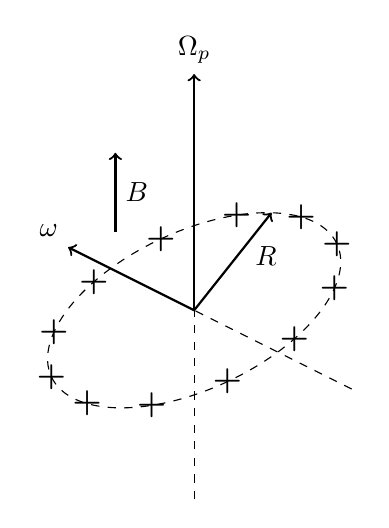
\begin{tikzpicture}[scale=2]

% Parametri ellisse
\def\a{1}   % semiasse maggiore
\def\b{0.5} % semiasse minore
\def\rot{25} % angolo di rotazione in gradi

% Ellisse inclinata corretta
\begin{scope}[rotate=\rot]
    \draw[dashed] (0,0) ellipse (1 and 0.5);
\end{scope}

% Cariche positive distribuite lungo ellisse inclinata
\foreach \angle in {0,30,...,345} {
    \pgfmathsetmacro{\x}{\a*cos(\angle)*cos(\rot) - \b*sin(\angle)*sin(\rot)}
    \pgfmathsetmacro{\y}{\a*cos(\angle)*sin(\rot) + \b*sin(\angle)*cos(\rot)}
    \node at (\x,\y) {\textbf{\large +}};
}

% Linea verticale tratteggiata (Omega_p)
\draw[dashed] (0,-1.2) -- (0,1.5);
\draw[->,thick] (0,0) -- (0,1.5) node[above] {$\Omega_p$};

% Freccia omega inclinata verso l'alto (effetto 3D)
\draw[->,thick] (0,0) -- (-0.8,0.4) node[above left] {$\omega$};
\draw[dashed] (1,-0.5) -- (0,0);

% Vettore B (verticale)
\draw[->,thick] (-0.5,0.5) -- (-0.5,1) node[midway,right] {$B$};

% Raggio R (dall'origine verso bordo ellisse)
\pgfmathsetmacro{\Rx}{\a*cos(45)*cos(\rot) - \b*sin(45)*sin(\rot)}
\pgfmathsetmacro{\Ry}{\a*cos(45)*sin(\rot) + \b*sin(45)*cos(\rot)}
\draw[->,thick] (0,0) -- (\Rx,\Ry) node[pos=0.3, above right, xshift=10pt, yshift=2pt] {$R$};

\end{tikzpicture}